\documentclass{beamer}

\usepackage[UTF8,noindent]{ctexcap}
\usepackage{color}%引入颜色
\usetheme{Warsaw}
\usecolortheme{seahorse}
\usepackage{graphicx}%引入插图
\usepackage{ulem}%删除线
\usepackage{tikz}  
\usetikzlibrary{arrows.meta}%画箭头用的包

\usefonttheme[onlymath]{serif}

\usepackage{graphicx}
\usepackage{subfigure}
\usepackage{amsmath}
\usepackage{tabularx}
\usepackage{color}
\usepackage{hyperref}
\usepackage{ulem}
\usepackage{multirow}
\hypersetup{
	colorlinks=true,
	linkcolor=black
}

\usepackage[cache=false]{minted}
\usepackage{multirow}

\usepackage{algorithm}
\usepackage{algorithmicx}
\usepackage{algpseudocode}
\usepackage{amssymb}
\usepackage{qcircuit}
\usepackage{fancyhdr}
\usepackage{cleveref}
\usepackage{tikz}  

\useoutertheme{infolines}
%\usepackage[orientation=landscape,size=custom,width=16,height=9,scale=0.5,debug]{beamerposter}

\def \ket#1{|#1 \rangle}
\def \bra#1{\langle #1|}
\def \braket#1#2{\langle #1|#2\rangle}


\title{Isotonic Regression}
\date{2021年12月22日}
\author{信息科学技术学院\ \ \ 周书予}

%\setbeamercovered{dynamic}
\begin{document}\small
	
%\usebackgroundtemplate{\tikz\node[inner sep=0pt,opacity=0.3]{\includegraphics[width=16cm,height=9cm]{zsy_background.jpg}};}
	\begin{frame}
	\titlepage
	\end{frame}
\section{Q \& A}
\begin{frame}{Q \& A}
\begin{itemize}
	\item Q: 什么是Isotonic Regression?\pause
	\item A: Isotonic Regression就是保序回归(确信)。\pause
	\item Q: 什么是保序回归?\pause
	\begin{itemize}
		\item Q: 什么是保序?\pause
		\item A: 大家都学过离散/集图了,就不解释了。\pause
		\item Q: 什么是回归?\pause
		\item A: 大家都炼过丹了,就不解释了。		\pause
	\end{itemize}
	\item Q: 我知道保序回归是什么意思了,但是你是谁?\pause
	\item A: 这不重要。
\end{itemize}
\end{frame}
\section{问题描述}
\begin{frame}{问题描述}
\begin{block}{Definition}
	给定偏序集$\mathcal X$以及$\mathcal X$上的函数$y: \mathcal X \to \mathbb R, w: \mathcal X \to \mathbb R^+$。定义一个函数$z: \mathcal X \to \mathbb R$是保序的,如果$\forall a, b \in \mathcal X,  a \preceq b \Rightarrow z_a \le z_b$。最优化问题
	$$L_p(\mathcal X, y, w) = \min_{z}\begin{cases}
	\sum_{a \in \mathcal X}w_a|y_a - z_a|^p, & 1 \le p < \infty\\
	\max_{a \in \mathcal X}w_a|y_a - z_a|, & p = \infty
	\end{cases}, s.t.\ z\ \mbox{是保序的}$$
	被称为$L_p$保序回归问题,简称$L_p$问题。
\end{block}
\pause
$p = \infty$处的定义是自然的。
\end{frame}
\iffalse
\section{P0}
\begin{frame}{热身题}
\begin{block}{Statement}
	一般偏序集$\mathcal X$上保证$w_a \equiv 1$的$L_{\infty}$问题?
\end{block}\pause
\begin{block}{Tutorial}
	$$L_{\infty}(\mathcal X, y, \mathbf 1) = \max_{a \in \mathcal X}\left\{ \left(\max_{b \preceq a} y_b - \min_{a \preceq c} y_c\right) / 2\right\}$$\pause
	
	答案至少是这个值: 显然。\pause
	
	答案可以取这个值: 取$z_a = \left(\max_{b \preceq a} y_b + \min_{a \preceq c} y_c\right) / 2$即可。
\end{block}
\end{frame}
\fi
\section{P1}
\begin{frame}{可能是热身题}
\begin{block}{Statement}
	$\mathcal X$形如一条链。$p = 2$。
	
	或者等价的,给出序列$\{y_i\}_{i=1}^{n}, \{w_i\}_{i=1}^{n}$,需要构造\textbf{递增}序列$\{z_i\}_{i=1}^{n}$,最小化
	$$\sum_{i=1}^{n} w_i(y_i - z_i)^2$$
\end{block}
\pause
如果$y_i$递增?

\end{frame}

\begin{frame}{可能是热身题}
\begin{block}{Lemma}
	如果存在$y_i > y_{i+1}$,则最优的$z$一定满足$z_i = z_{i+1}$。	
\end{block}
\pause
一旦出现$y_i > y_{i+1}$,就可以把$i$和$i+1$合并,得到$y' = \frac{y_iw_i + y_{i+1}w_{i+1}}{w_i + w_{i+1}}$和$w' = w_i + w_{i+1}$,用$(y', w')$替换$(y_i, w_i), (y_{i+1}, w_{i+1})$。\\

重复合并直至$y_i$递增。\\\pause

实现上可以用单调栈维护合并,复杂度为$O(n)$。

\end{frame}

\section{P2}
\begin{frame}{忘记写标题了}
\begin{block}{Statement}
	$\mathcal X$形如一棵树。$p = 1$。
\end{block}\pause

一种思路是动态规划,记$dp_{i, j}$表示确定$i$子树的取值且$i$节点取值为$j$的最小代价。\pause\\

注意到$dp_{i, j}$是关于$j$的线性分段凸函数(斜率递增),可以用线段树维护$dp$数组,转移时需要实现线段树合并。\\

\sout{不讨论实现细节。}

\end{frame}

\section{P3}
\begin{frame}{整体二分的引入}
	整体二分是OI中常见的用于处理多组二分询问的算法,核心思路是通过整体性的预处理以避免信息的重复计算,或者维护必要的限制条件。\pause	

	然后我们引入一些约定。\pause
	\begin{block}{Definition}
	将序列$z$中不大于$a$的元素变成$a$,不小于$b$的元素变成$b$,称这个过程为$z$向$S = \{a, b\}$取整。
\end{block}
\pause
\begin{block}{Definition}
	对于一个$L_p$问题,定义$L_p^{S}$问题为把$z_i$取值限定在$S$内的原$L_p$问题。
\end{block}\pause
\begin{block}{Definition}
	$\mathcal X$的一个子集$\mathcal U$的$L_p$-mean定义为$\min\limits_{k \in \mathbb R}\begin{cases}
	\sum_{a \in \mathcal U} w_a|y_a - k|^p, & 1 \le p < \infty\\
	\max_{a \in \mathcal U} w_a|y_a - k|, & p = \infty
	\end{cases}$。
	
\end{block}

\end{frame}

\begin{frame}{$p = 1$}
	\begin{block}{Lemma}
		$L_1$问题一定存在一组最优解$z$,满足$z_i \in \{y_1, y_2, \cdots, y_n\}$。
	\end{block}
	\pause
	\begin{block}{Theorem}
	在一个$L_1$问题中,若所有$y_i$都不在$(a, b)$中,记$z^S$表示$L_1^S$问题的一组最优解,那么一定存在一组$L_1$满足$z_i \notin (a, b)$的最优解$z$,使得$z$向$S$取整可以得到$z^S$。
	\end{block}

\end{frame}

\begin{frame}{$p = 1$}
	\begin{block}{Theorem}
	在一个$L_1$问题中,若所有$y_i$都不在$(a, b)$中,记$z^S$表示$L_1^S$问题的一组最优解,那么一定存在一组$L_1$满足$z_i \notin (a, b)$的最优解$z$,使得$z$向$S$取整可以得到$z^S$。
	\end{block}
\begin{center}
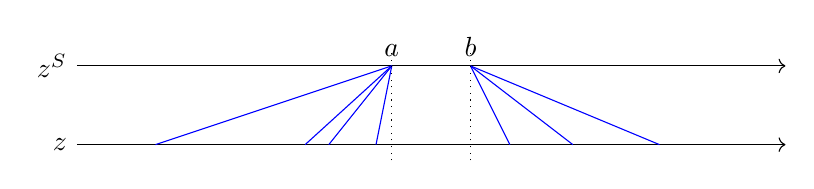
\begin{tikzpicture}

\coordinate (A) at (4, 1);
\coordinate (B) at (5, 1);

\draw[->] (0, 0)--(9, 0);
\draw[->] (0, 1)--(9, 1);
\draw (0, 0) node [left]{$z$};
\draw (0, 1) node [left]{$z^S$};
\draw (A) node [above]{$a$};
\draw (B) node [above]{$b$};

\draw [color=blue] (1, 0)--(A);
\draw [color=blue] (2.9, 0)--(A);
\draw [color=blue] (3.2, 0)--(A);
\draw [color=blue] (3.8, 0)--(A);

\draw [color=blue] (5.5, 0)--(B);
\draw [color=blue] (6.3, 0)--(B);
\draw [color=blue] (7.4, 0)--(B);

%\draw [color=red] (2.5, 0)--(B);
%\draw [color=red] (5.2, 0)--(A);

\draw[dotted] (4, -0.2)--(4, 1.2);
\draw[dotted] (5, -0.2)--(5, 1.2);

\end{tikzpicture}
\end{center}

证明?\pause 反证,先陈述否命题:任意一组$L_1$满足$z_i \notin (a, b)$的最优解$z$,都存在$j$使$z_j \le a, z_j^S = b$,或者$z_j \ge b, z_j^S = a$。\\

注意到两种情况是不可能同时出现的,所以不失一般性地只考虑出现前者。

\end{frame}

\begin{frame}{大讨论}
\begin{center}
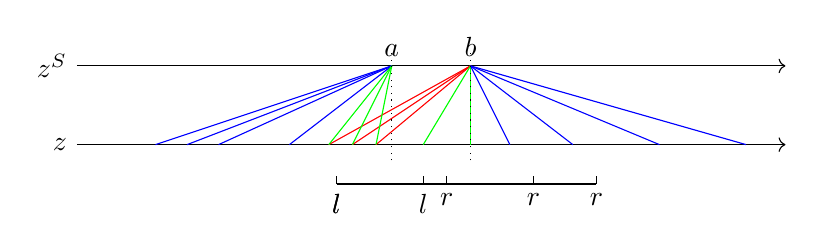
\begin{tikzpicture}

\coordinate (A) at (4, 1);
\coordinate (B) at (5, 1);

\draw[->] (0, 0)--(9, 0);
\draw[->] (0, 1)--(9, 1);
\draw (0, 0) node [left]{$z$};
\draw (0, 1) node [left]{$z^S$};
\draw (A) node [above]{$a$};
\draw (B) node [above]{$b$};

\draw [color=blue] (1, 0)--(A);
\draw [color=blue] (1.4, 0)--(A);
\draw [color=blue] (1.8, 0)--(A);
\draw [color=blue] (2.7, 0)--(A);

\onslide<1-2,4,6>{
	\draw [color=red] (3.2, 0)--(B);
	\draw [color=red] (3.5, 0)--(B);
	\draw [color=red] (3.8, 0)--(B);
}

\onslide<3>{
	\draw [color=green] (4.4, 0)--(B);
}
\onslide<5>{
	\draw [color=green] (5,0)--(B);
}
\onslide<7>{
	\draw [color=green] (3.2, 0)--(A);
	\draw [color=green] (3.5, 0)--(A);
	\draw [color=green] (3.8, 0)--(A);
}

\draw [color=blue] (5.5, 0)--(B);
\draw [color=blue] (6.3, 0)--(B);
\draw [color=blue] (7.4, 0)--(B);
\draw [color=blue] (8.5, 0)--(B);

\draw[dotted] (4, -0.2)--(4, 1.2);
\draw[dotted] (5, -0.2)--(5, 1.2);

\onslide<2-3>{
	\coordinate (L) at (4.4, -0.5);
	\coordinate (LL) at (4.4, -0.4);
	\coordinate (R) at (5.8, -0.5);
	\coordinate (RR) at (5.8, -0.4);
	
	\draw (L)--(R);
	\draw (L)--(LL);
	\draw (R)--(RR);
	\draw (L) node [below]{$l$};
	\draw (R) node [below]{$r$};
}

\onslide<4-5>{
	\coordinate (L) at (3.3, -0.5);
	\coordinate (LL) at (3.3, -0.4);
	\coordinate (R) at (6.6, -0.5);
	\coordinate (RR) at (6.6, -0.4);
	
	\draw (L)--(R);
	\draw (L)--(LL);
	\draw (R)--(RR);
	\draw (L) node [below]{$l$};
	\draw (R) node [below]{$r$};
}

\onslide<6-7>{
	\coordinate (L) at (3.3, -0.5);
	\coordinate (LL) at (3.3, -0.4);
	\coordinate (R) at (4.7, -0.5);
	\coordinate (RR) at (4.7, -0.4);
	
	\draw (L)--(R);
	\draw (L)--(LL);
	\draw (R)--(RR);
	\draw (L) node [below]{$l$};
	\draw (R) node [below]{$r$};
}


\end{tikzpicture}
\end{center}

把“不好”的集合记作$U$,考虑$U$的$L_1$均值的取值区间\footnote{\tiny 可能退化成一个点。}$[l, r]$。\\

\onslide<2-3>{
	Case 1: $a \le l.$
	\onslide<3>{
		此时把$U$中元素的$z_i$都改成$\min\{l, b\}$,就能使结果严格变优,同时没有破坏原有偏序结构,于是$z$的最优性假设就寄了。
	}
}

\onslide<4-5>{
	Case 2: $l \le a, b \le r.$
	\onslide<5>{
		此时把$U$中元素的$z_i$都改成$b$,结果一定不会变劣,而又在没有破坏原有偏序结构的情况下构造出了“好”的情况,于是“不存在”的假设就寄了。
	}
}

\onslide<6-7>{
	Case 3: $l \le a, r < b.$
	\onslide<7>{
		此时把$U$中元素的$z_i^S$都改成$a$,结果严格变优,偏序结构也没有破坏,于是$z^S$的最优性假设就寄了。
	}
}

\end{frame}

\begin{frame}[fragile]{总之就是非常对,并且扩展到任意$p < \infty$都是对的}
	前面我们说过了,对于$L_1$问题,一定存在一组最优解$z$,其中每个元素的取值都是某个出现过的$y_i$值。\\
	
	于是$z$的取值集合大小不超过$n$,只需要在这个集合上整体二分就可以了。\\\pause
	
	这样的性质在$p > 1$时不再满足。\pause 不过我们有另一个结论。
	
	\begin{block}{Lemma}
		$p > 1$时,任意集合的$L_p$-mean是唯一的。
	\end{block}\pause
	
	由于$X$有限,其所有子集的$L_p$-mean取值范围也有限,故对于任意$a \in \mathbb R$,总能找到$\varepsilon > 0$使得$(a, a + \varepsilon)$内没有最优解里的元素。\\\pause
	
	此时欲做$L_p^{\{a, a + \varepsilon\}}$问题,相比于比较$z_i$取$a$与取$a + \varepsilon$的差值(太小了!),可以考虑求代价函数在$a$处的导数作为替代。
	
\end{frame}
\begin{frame}{算法模板}
	以$p = 1$为例。\\
	
	\begin{algorithmic}[1]
		\Function{solve}{$\mathcal X$, $Y$}
			\If{$|Y| = 1$ or $\mathcal X = \varnothing$}
				\State ...this case is trivial
			\Else
				\State $mid \gets \lceil \frac{|Y|}{2} \rceil$
				\State $a, b \gets $ the $mid$-th and $(mid+1)$-th smallest element in $Y$
				
				\State solve $L_1^S$ problem for $S = \{a, b\}$ and obtain $z^S$ 
				
				\State partition $\mathcal X$ into $\mathcal X_a, \mathcal X_b$ via $z^S$
				
				\State \Call{solve}{$\mathcal X_a$, first $mid$ elements in $Y$}
				
				\State \Call{solve}{$\mathcal X_b$, last $(|Y| - mid)$ elements in $Y$}
				
			\EndIf
		\EndFunction
	\end{algorithmic}
	
\end{frame}

\begin{frame}{某校内胡策题}
	\begin{block}{Statement}
		给定一张 $n$ 个点 $m$ 条边的无向连通图 $G = (V, E)$ 和边集 $E_1, E_2 \subseteq E$,每条边有初始权值 $d_i$,定义一次操作为把一条边的权值加 $1$ 或减 $1$ ,求至少需要多少次操作可以使
		\begin{itemize}
			\item 边集$E_1$是整张图的一棵最小生成树;
			\item 边集$E_2$是整张图的一棵最大生成树。
		\end{itemize}
	\end{block}
\end{frame}

\begin{frame}{拟阵?}
	不加证明地引用\cite{p2}中的一个结论
	\begin{block}{Theorem(强基交换定理)}
		对于拟阵$M$,假设存在两个不同的基$A, B$,那么对于任意一个元素$x \in A \setminus B$,都存在一个元素$y \in B \setminus A$,满足$A \setminus \{x\} \cup \{y\}$和$B \setminus \{y\} \cup \{x\}$都是拟阵的基。
	\end{block}\pause
	
	同样不加证明地声称最小/大生成树是拟阵,并且指出题目中要求的条件成立当且仅当
	\begin{itemize}
		\item $\forall e' \in E \setminus E_1$,若其可以替换$E_1$上的一条边$e$,则$w_{e'} \ge w_e$;$E_2$同理。
	\end{itemize}

	\pause
	
	这样就把原问题转化成了保序回归问题,套用前面说过的方法就可以解决了。
	
\end{frame}

\begin{frame}{是不是有什么忘了讲了}
	我们好像还没有说$L_p^S$问题咋做...\\
	
	$L_p \to L_p^S$的规约把问题从回归转化成了$2$分类,但此时仍需要考虑偏序关系。\pause \\
	
	(摆烂讲法)$a \preceq b$视作$a \to b$的一条有向边,此时需要在建出的图中找出一个闭合子图并让其取$S$中较大的值,同时还要求最小代价,可以使用网络流解决。
\end{frame}

\begin{frame}{你已经完全掌握这个算法了,来看一道省选题吧}
	\begin{block}{「联合省选 2020 A」魔法商店}
		有$n$件标有「价格」和「魅力值」的商品。
		
		定义一个商品集合是「好」的,如果其任意子集「魅力值」异或和不为$0$,同时集合大小是满足前者时最大的。
		
		可以以$(v - v')^2$的代价把一件商品的「价格」从$v$修改成$v'$。\textbf{只能改成整数}。
		
		要求最小化总代价,使最终给定集合$A$是「价格」和最小的「好」的集合,集合$B$是「价格」和最大的「好」的集合。
	\end{block}
\pause
$\mathbb F_2$上线性空间也是拟阵...

\end{frame}
\begin{frame}{周歪歪的序列}
	\begin{block}{Statement}
		有一个长度为 $N$ 的序列以及 $M$ 个形如“第$k$个数是区间$[l, r]$内最小/大的数”限制。
		
		你需要尽量少地修改序列, 使得序列满足限制。“尽量少”指的是最小化所有元素的变化量之和。
	\end{block}\pause

	有没有比网络流更快的实现$2$分类的算法呢?\pause\\
	
	动态规划,$dp_{i, 0/1}$表示前$i$个元素已经完成分类时,且第$i$个元素分在第$0/1$类的最小代价。\\
	
	转移使用线段树优化。\\
	
	具体实现细节可以询问出题人(雾
\end{frame}
\section{P4}
\begin{frame}{$p = \infty$}
	$p = \infty$时,前述做法不再适用了。\pause\\
	
	但实际上$p = \infty$的问题比$p < \infty$要更(自然语言意义上的)简单。考虑$$\mathrm{minimize}\ \max_{a \in \mathcal X}w_a|y_a - z_a|$$
	
	\pause “最小化最大值”可以尝试用二分来解决。\\
	
	\pause 二分结果,从而为每个$a \in \mathcal X$确定可行的取值范围。\\
	
	按照$\mathcal X$的拓扑序依次确定每个$z_a$的取值。贪心是正确的。
\end{frame}

\section{Reference}
\begin{frame}{Reference}
\bibliographystyle{unsrt}
\bibliography{ref}
\end{frame}



\end{document}